\newpage

\section*{Приложение}%

{\bf А. Дополнительный функционал}

Добавлен новый функционал приложения:
\begin{itemize}
	\item при нажатии "в процессе" у занятой книги появляется соответствующее уведомление с именем пользователя, у которого находится книга;
	\item на главной и поисковой страницах отображается то, что книга занята и кем;
	\item незарегистрированный пользователь может просматривать содержимое библиотеки и пользоваться поиском.
\end{itemize}

\begin{lstlisting}[label=some-code, caption=Новые функции класса Status]
def check_status_equal_two(book_id):
        conn = sqlite3.connect("app.db")
        cursor = conn.cursor()
        cursor.execute("select S.status, username \
                        from ( \
                                select status, user_id \
                                from status \
                                where book_id = (?) and status = 2 \
                            ) as S join user on S.user_id = user.id \
                             where id != (?);", (book_id, current_user.id))
        res = cursor.fetchone()
        conn.close()
        return res


    def check_all_status_equal_two():
        conn = sqlite3.connect("app.db")
        cursor = conn.cursor()
        cursor.execute("select S.status, username, S.book_id \
                        from ( \
                            select status, user_id, book_id \
                            from status \
                            where status = 2 \
                            ) as S join user on S.user_id = user.id;") 
        res = cursor.fetchall()
        conn.close()
        return res
\end{lstlisting}


\begin{figure}[H]
\center{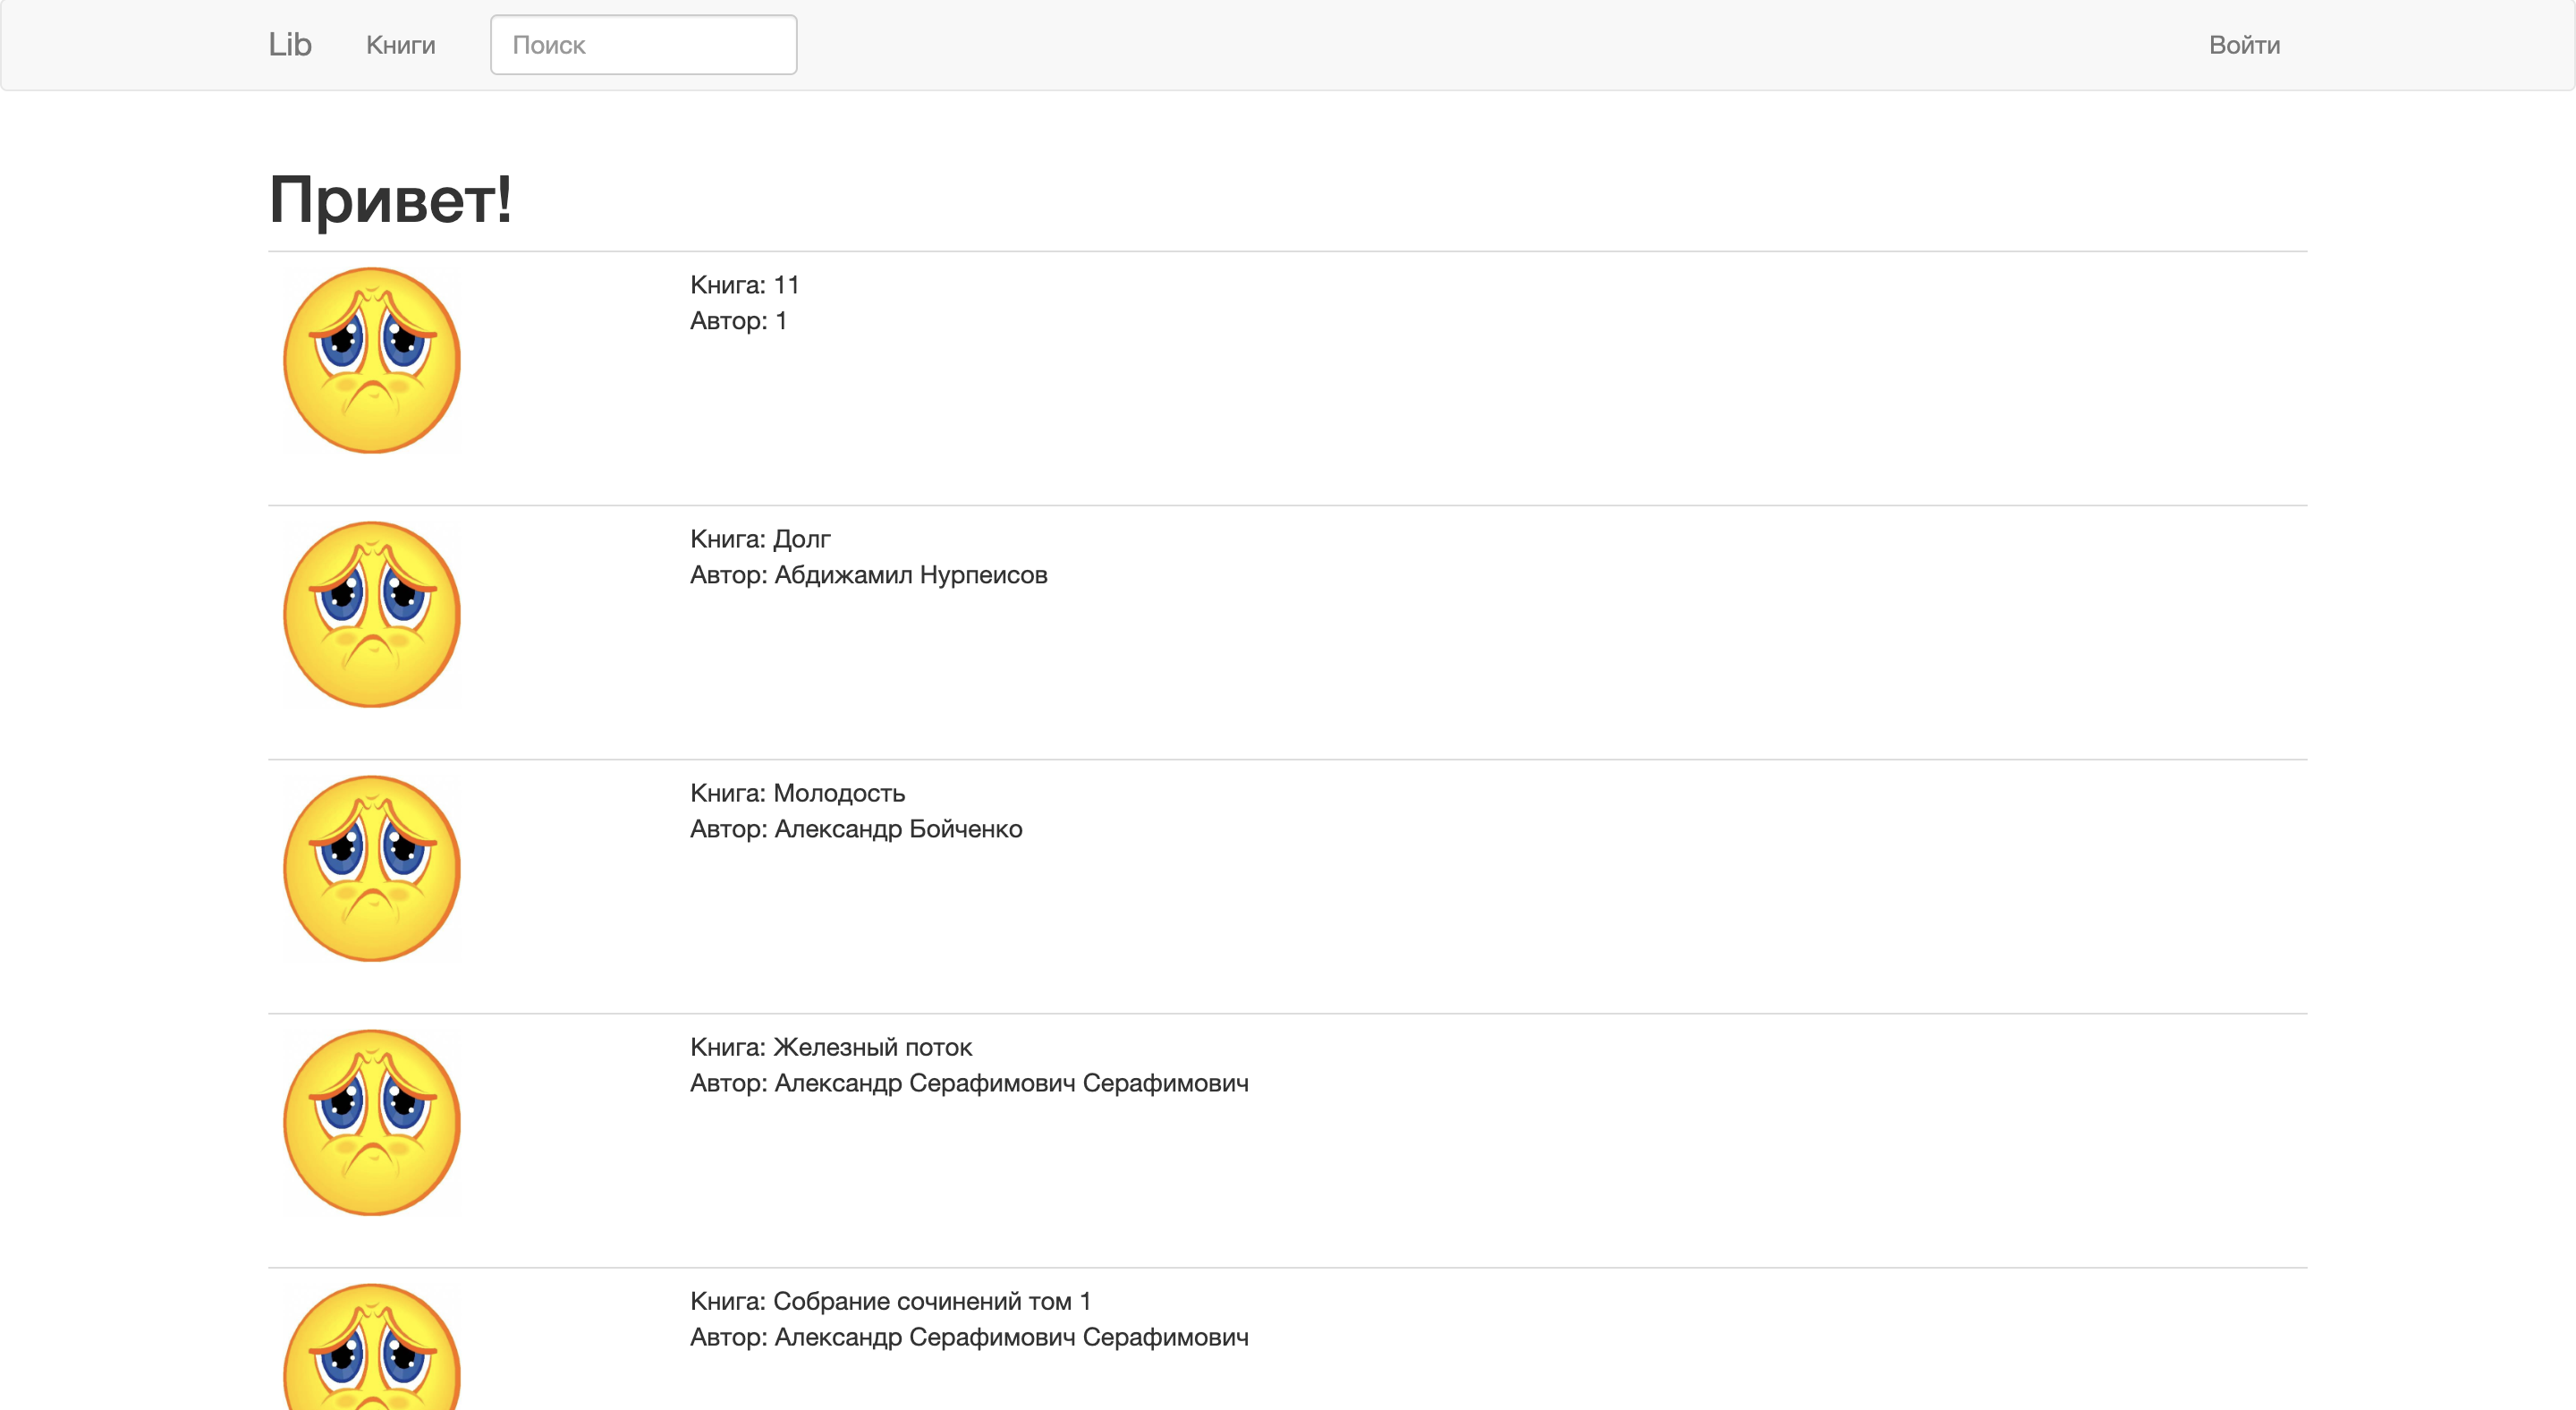
\includegraphics[scale=0.3]{p1.png}}
\caption{Вид главной страницы для неавторизованного пользователя}
\label{fig:image}
\end{figure}

\begin{figure}[H]
\center{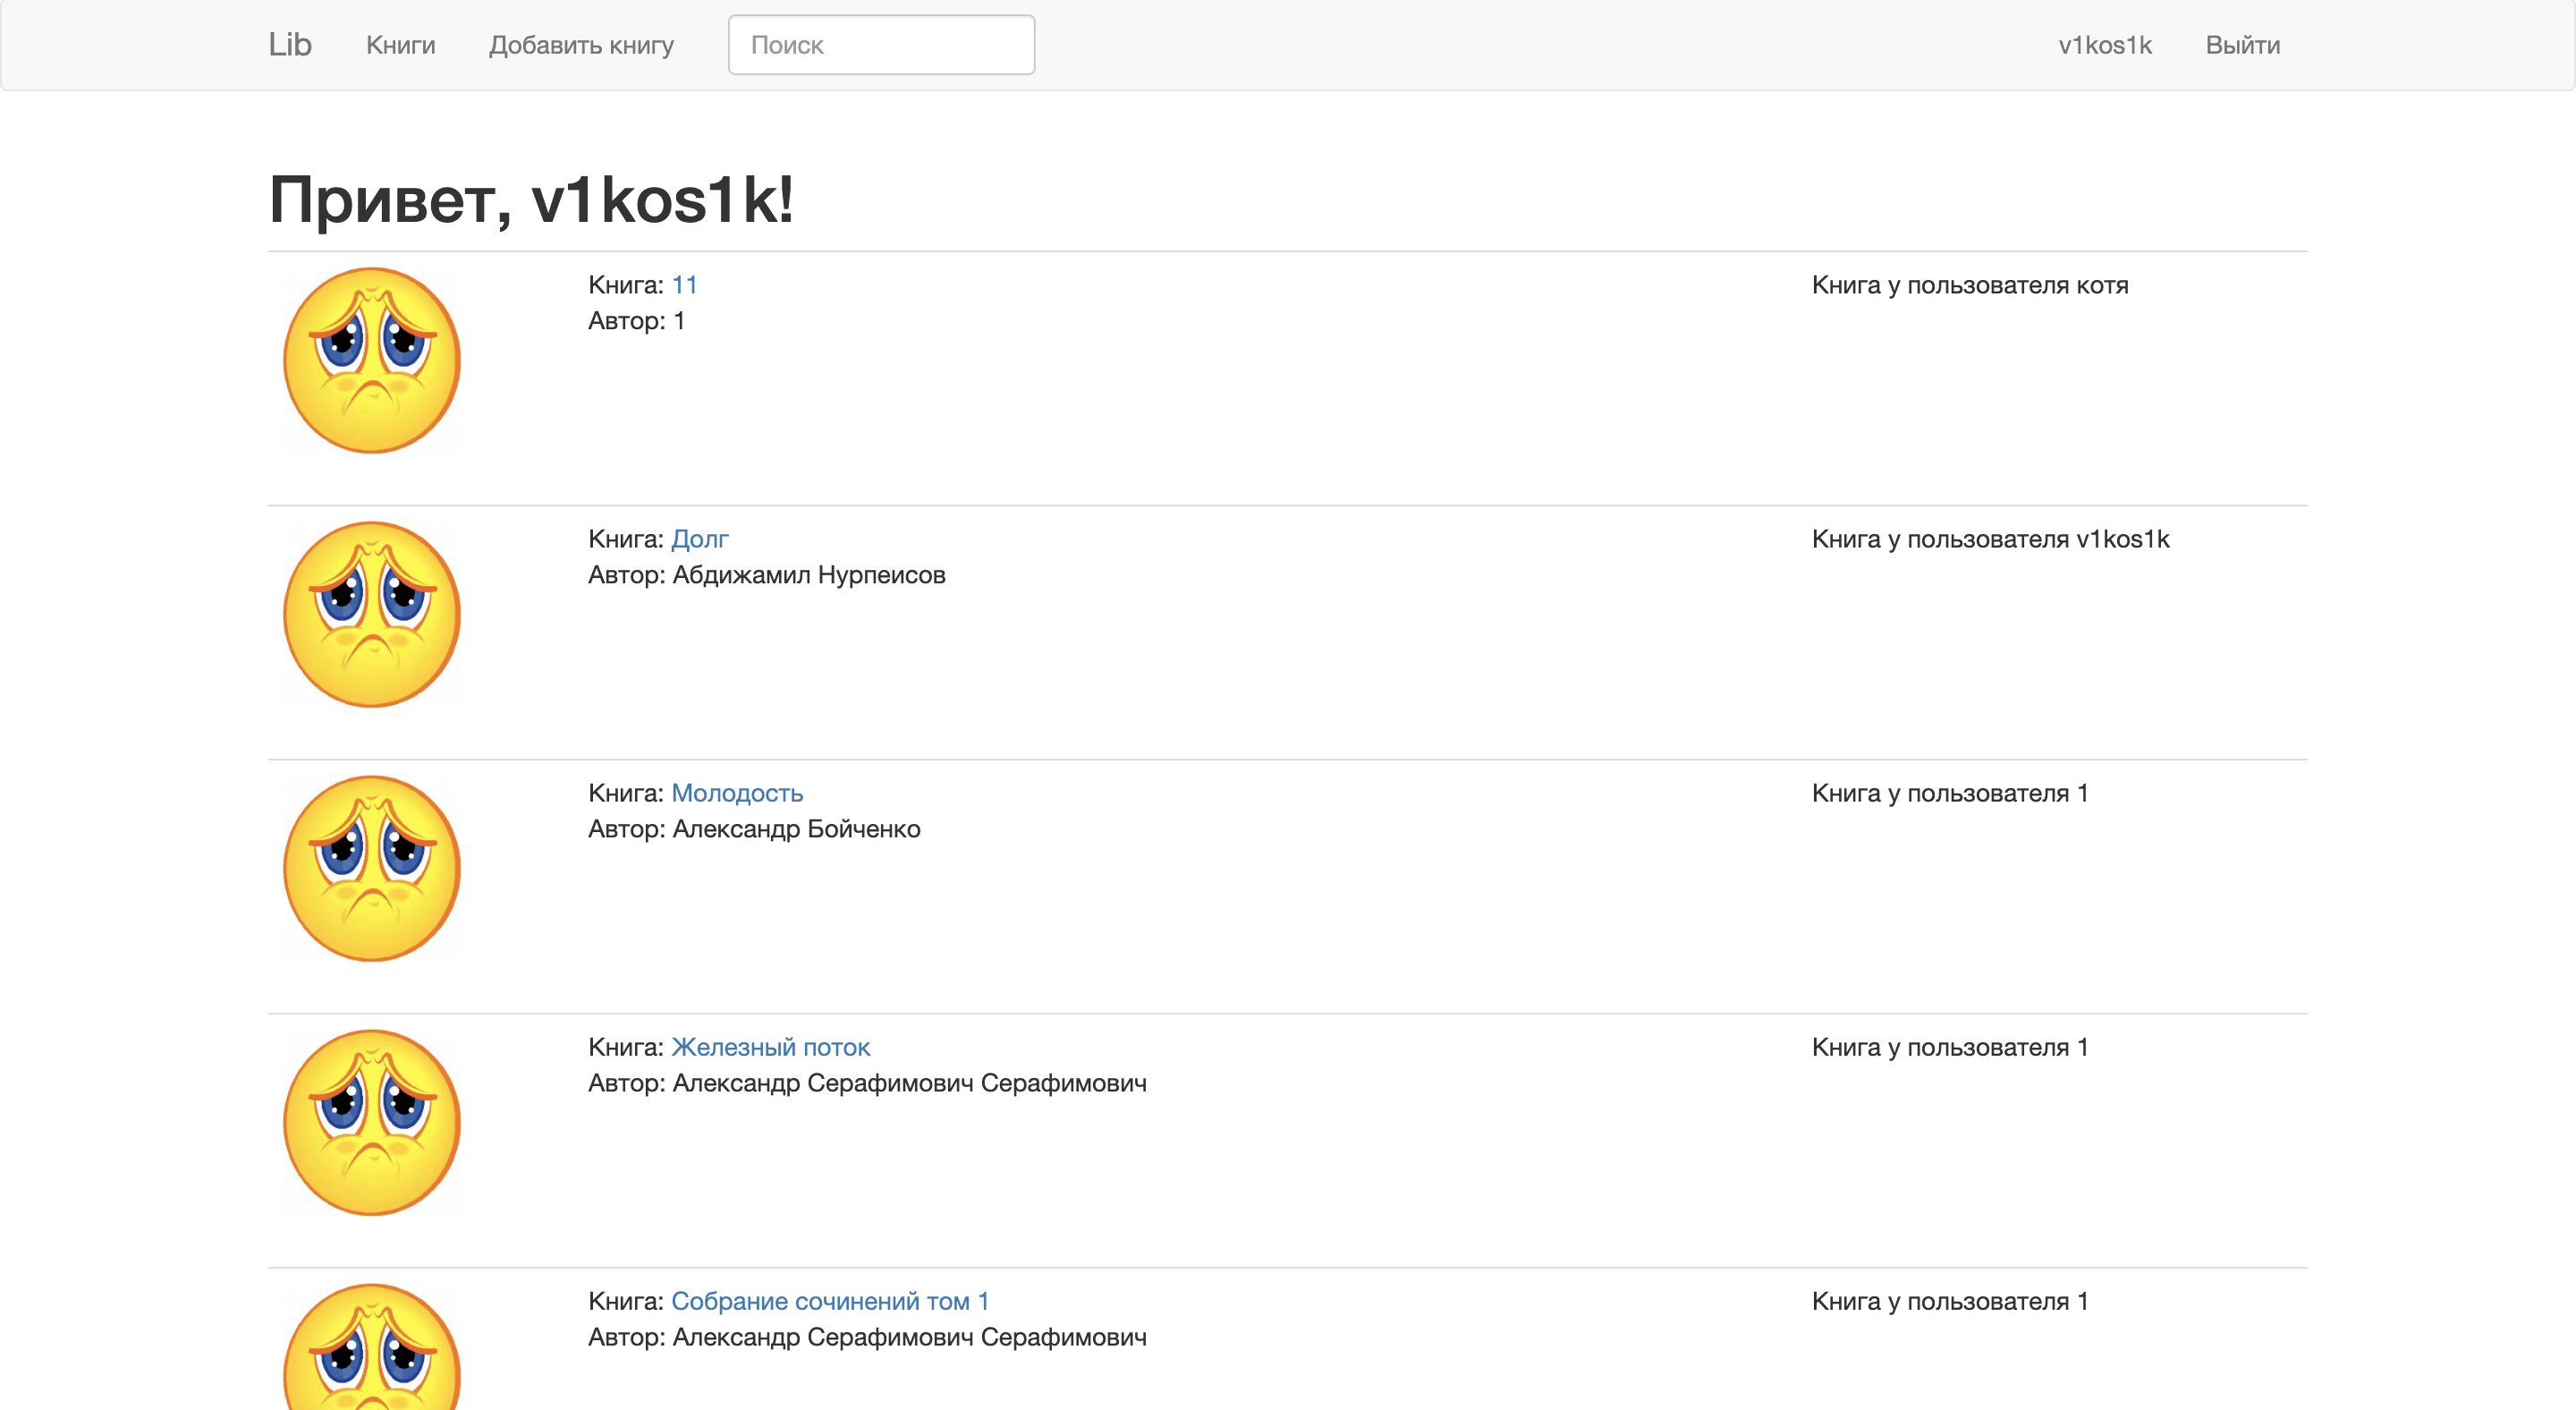
\includegraphics[scale=0.3]{p2.png}}
\caption{Вид главной страницы для авторизованного пользователя}
\label{fig:image}
\end{figure}

\begin{figure}[H]
\center{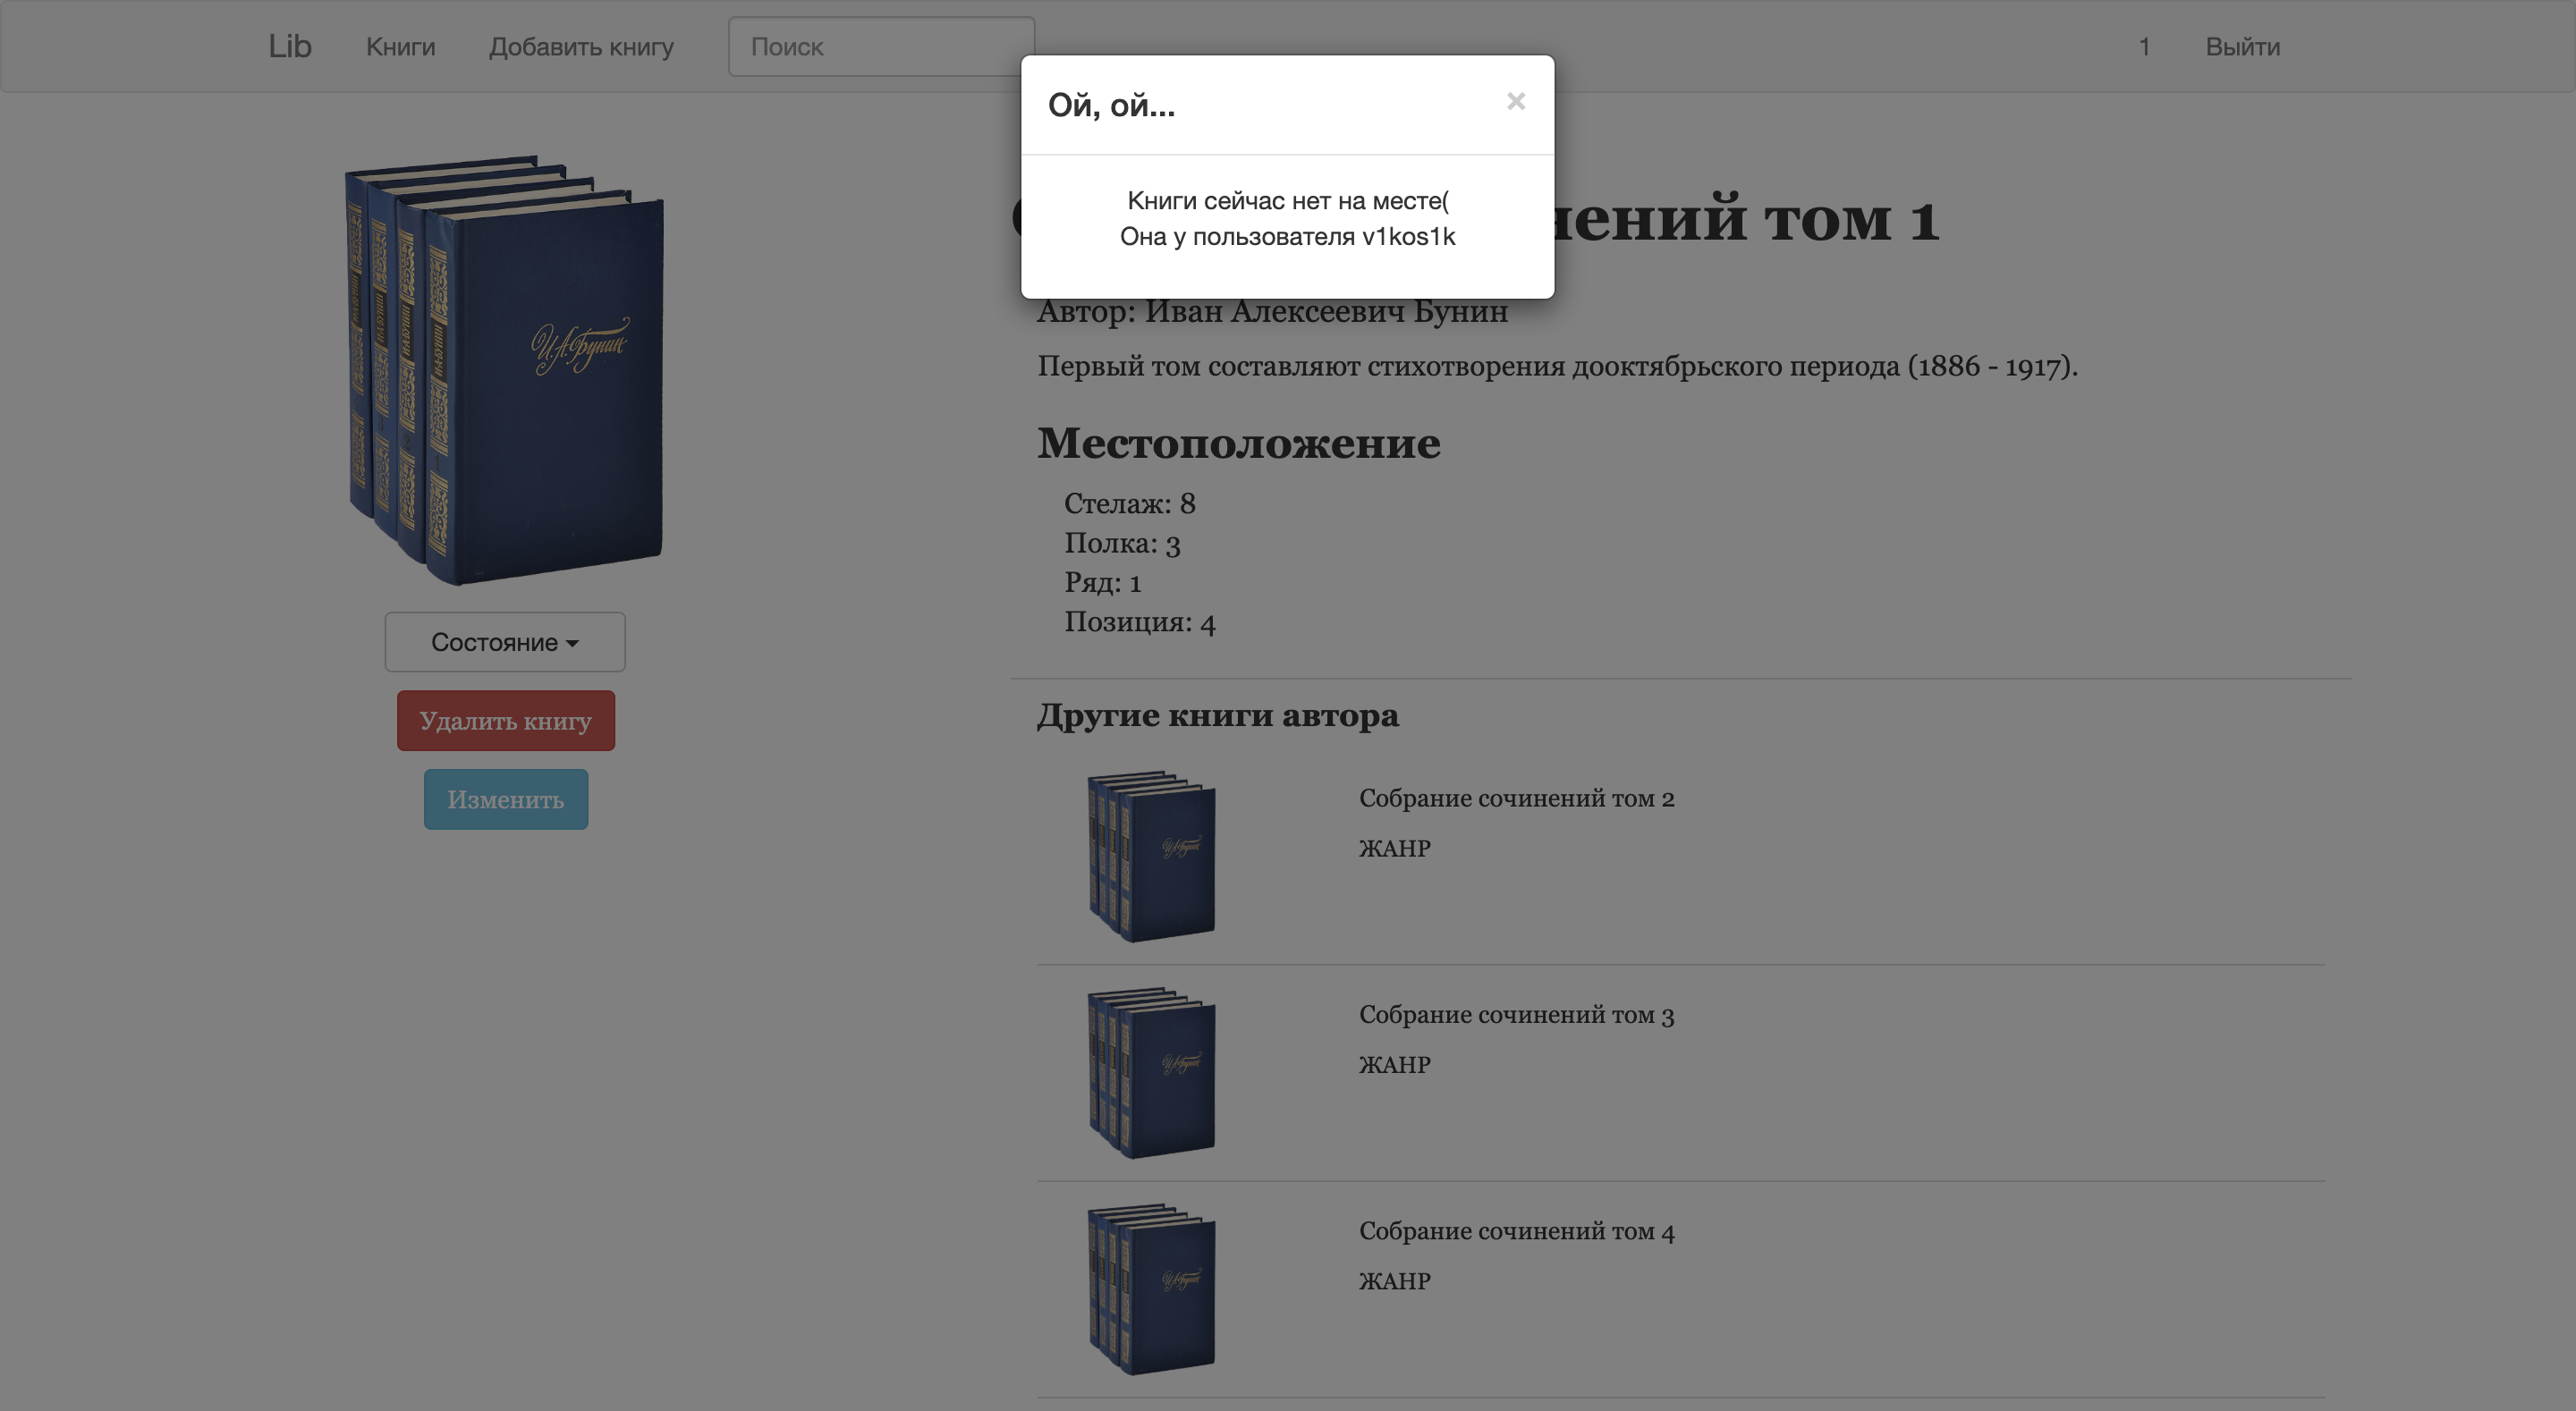
\includegraphics[scale=0.3]{p3.png}}
\caption{Пример попытки добавления занятой книги}
\label{fig:image}
\end{figure}

\begin{figure}[H]
\center{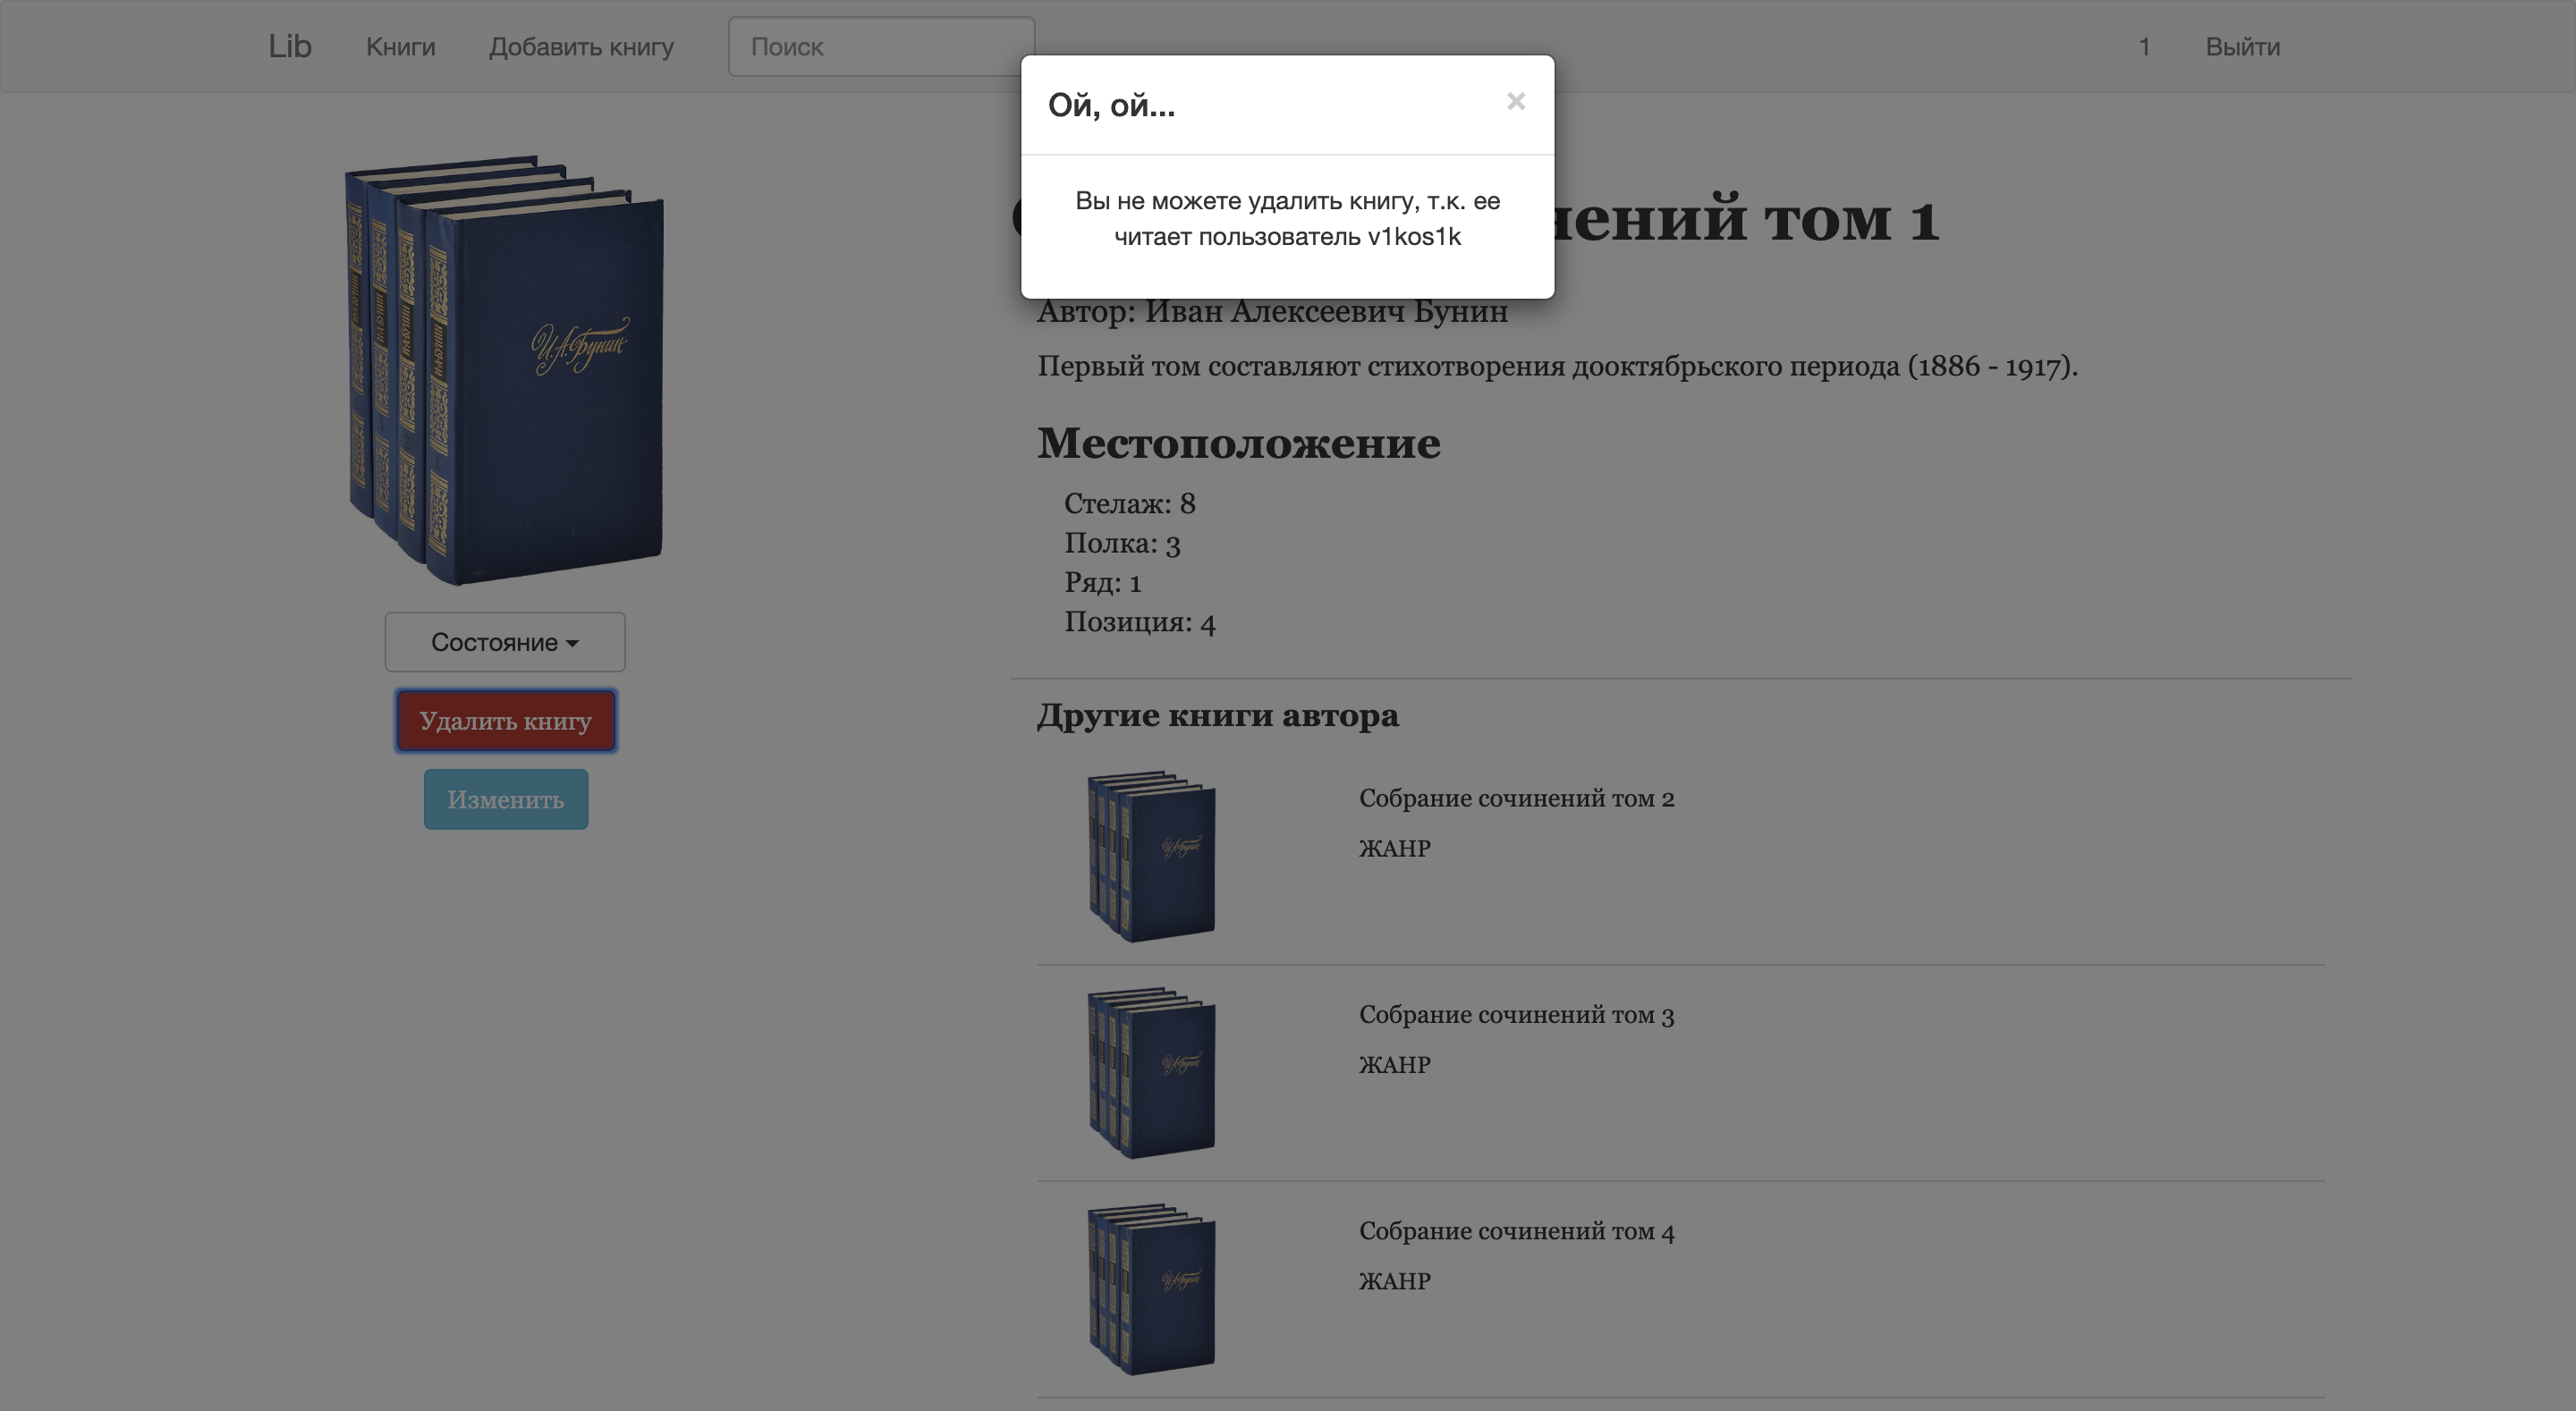
\includegraphics[scale=0.3]{p4.png}}
\caption{Пример попытки удаления занятой книги}
\label{fig:image}
\end{figure}





















